% !TeX spellcheck = de_DE
In diesem Kapitel wird das bestehende Projekt aus nachvollzogen und überarbeitet. Inhalte sind das Testen bestehender Vorlagen aus \cite{wirthErweiterungBestehendenDrohne2022} und \cite{wirthErweiterungBestehendenDrohne2022a}, sowie das Aufsetzen einer neuen Arbeitsumgebung wie in beschrieben in \cite{haraldwirthNachfolgerInfoStudienarbeitAutonome2022}, siehe \cref{chap:nachfolger}.

\section{Inbetriebnahme}\label{chap:einarbeite}
Zur Aufarbeitung des Projektes steht ist die Drohne bestehend aus Rahmen, Flugcontroller, Motoren mit Propellern, Ultraschallsensoren und Akku bereit. Nicht vorhanden sind die RC-Fernsteuerung und der auf die Drohne montierte \gls{rpi}. Ursprünglich verwedet wurde ein \gls{rpi} 4 Model B mit $2GB$ \gls{ram} als Bordcomputer, der mit dem Flugcontroller kommuniziert, dessen Daten über ein Netzwerk verbreitet und auch Anweisungen zum Flug geben kann. Gleiches kann auch mit dem \gls{rpi} 3 Model B+ bewerkstelligt werden. Dieser bestitzt im Gegensatz nur 1GB \gls{ram} und weniger Rechenleistung.
Die gelieferte SD-Karte enthält das Betriebssystem Raspbian OS in der Ausführung als 32-bit Betriebssystem. Sowohl \gls{rpi} Model 4 als auch Model 3 besitzen zwar 64-bit Prozessoren, allerdings wird bei bis zu 4GB \gls{ram} das 32-bit Betriebssystem empfohlen um diesen effektiver auszunutzen.
Der verwendete \gls{rpi} startet somit problemlos.
Beim Systemstart wird automatisch der WLAN-Hotspot aktiviert und der MAVLINK-Server (mavlink-routerd) gestartet. %und verschiedene Docker Container
%Auf dem \gls{rpi} 3 führt dies führt zu einer hohen Systemauslastung, 1 von 4 CPU-Kernen ist permanent zu 100% belegt. Auch die Temperatur erhöht wodurch sich die Kerntemperatur auf ca 53°C erhöht. --- anscheinend doch nicht

\subsubsection{Verbindung Flugcontroller mit \gls{rpi}}
Durch das automatische Setup des \gls{rpi} sollte die Drohne mit dem Einstecken des Stromes bereit zum Flug sein. In \cite[Kapitel 4.3.6]{wirthErweiterungBestehendenDrohne2022} ist der erste Schritt beschrieben als "Test der Verbindung". Der \gls{rpi} wird mit dem Flugcontroller  per Serieller Schnittstelle verbunden (siehe auch \cref{chap:drone_coms}). Dazu wurde eigens ein Kabel entwickelt, welches die UART-Pins des \gls{rpi} mit dem TELEM2-Port des Flugcontrollers verbindet. Es ist zu beachten, dass keine Dokumentation bezüglich der Belegung der Kabeladern (per Jumper an den \gls{rpi} zu Stecken) gegeben ist. Ein Ausmessen des Kabels ergab:
\begin{compactitem}
    \item Schwarz: Masse -> Pin 06 des \gls{rpi}
    \item Braun: UART-Receive (Rx) des Flugcontrollers -> Pin 08 (Tx) des \gls{rpi}
    \item Weiß: UART-Transmit (Tx) des Flugcontrollers -> Pin 10 (Rx) des \gls{rpi}
\end{compactitem}
Anschließend soll die Verbindung wie in \cite[Kapitel 4.3.6]{wirthErweiterungBestehendenDrohne2022} beschrieben, die MAVLINK-Konsole geöffnet werden. Jedoch ist das Programm \textit{mavproxy} auf dem aktuellen Image nicht vorhanden. Um das weitere Vorgehen zu konkretisieren wurde das Programm nachinstalliert\footnote{\url{https://ardupilot.org/mavproxy/docs/getting_started/download_and_installation.html\#mavproxy-downloadinstalllinux}}. Das Starten des Konsolenprogrammes ist nur möglich, wenn der MAVLINK-Server (Prozess \textit{mavlink-routerd}) nicht läuft (ansonsten ist die Serielle Schnittstelle blockiert). Mit dem Befehl: 
\texttt{mavproxy.py -{}-master=/dev/serial0 -{}-baudrate=921600}
kann schließlich die Kommunikation des \gls{rpi} mit der Drohne verifiziert werden.

Für das weitere Vorgehen wird das allzeit vorliegende Programm \textit{mavlink-routerd} verwendet. Es arbeitet als Server im Hintergrund und verbreitet MAVLINK-Nachrichten im Netzwerk. Auch \textit{mavproxy} stellt solch eine Funktionalität bereit, allerdings wird aufgrund von zu erwartenden Leistungseinbußen davon abgeraten\footnote{\url{https://ardupilot.org/mavproxy/docs/getting_started/forwarding.html}}. Die Konfiguration des \textit{mavlink-routerd} wird wie in \ref{fig:mav_controller} dargestellt angepasst. Dadurch kann sich jedes Netzwerkgerät (auch der \gls{rpi} selbst) über das \gls{udp}-Protokoll mit dem Flugcontroller verbinden. Auch kann ein PC/ Smartphone eine Verbindung zum Flugcontroller über das Netzwerk herstellen. Mit der neuen Konfiguration steht sowohl ein TCP-Server, als auch ein UDP-Server zur Verfügung. Eine Auswertung zur Verwendung des geeignetsten Protokolls folgt in \cref{chap:bench_tcp_udp}. In Bild \ref{fig:mavconf_mavproxy} ist das Vorgehen zur Verbindung über einen Netzwerkknoten und das erneute Ausführen des Funktionstests dargestellt.

\begin{figure}
  \centering
    \subfloat[Alte Konfiguration von \texttt{mavlink-routerd}]{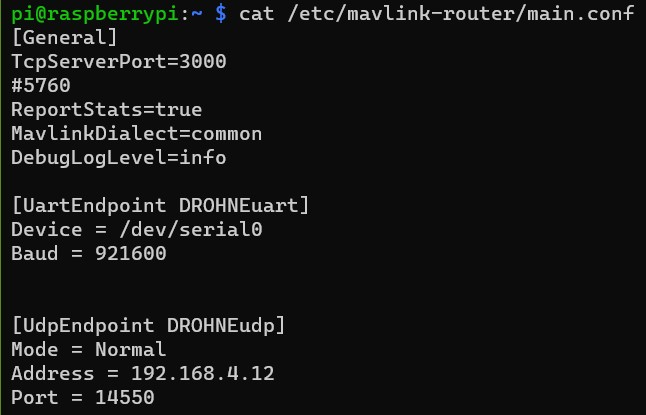
\includegraphics[width=0.5\textwidth]{images/mavlink.conf.old.jpg} \label{fig:mavconf_old}}
    \subfloat[BILD FALSCH, das ganze funktioniert anders! Neue Konfiguration von \texttt{mavlink-routerd}]{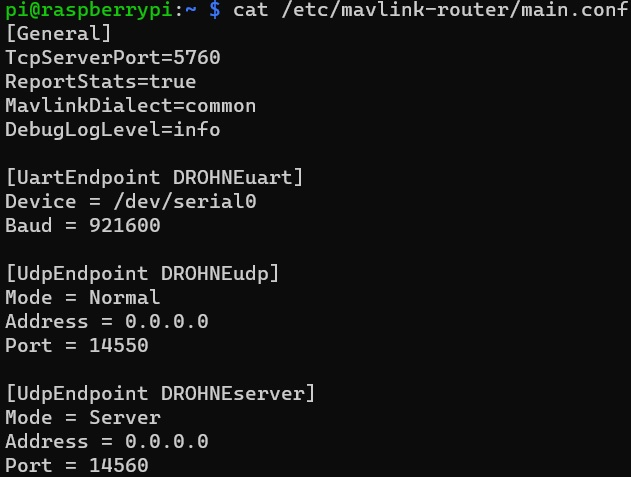
\includegraphics[width=0.5\textwidth]{images/mavlink.conf.new.jpg} \label{fig:mavconf_new}}
    
	\subfloat[Verbindung mittels \texttt{mavproxy} auf dem \gls{rpi}]{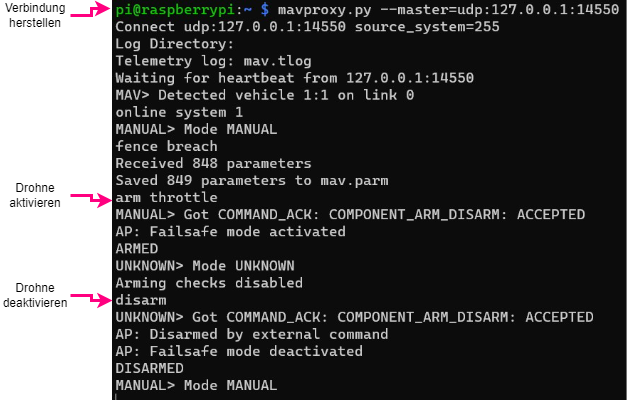
\includegraphics[width=0.8\textwidth]{images/mavlink_connect.png} \label{fig:mavconf_mavproxy}}
    
	\caption{Konfiguration und Verwendung von \texttt{mavlink-routerd}}
\label{fig:mav_controller}
\end{figure}

\subsubsection{Verbindung Flugcontroller mit PC}
Als \gls{gcs} zur Kommunikation mit dem Flugcontroller wird das Programm QGroundControl, wie in \cite[Kapitel 3.4]{wirthErweiterungBestehendenDrohne2022} vorgeschlagen, verwendet. Mit diesem können beliebige Drohnen konfiguriert, parametriert und geflogen werden. Der Flugcontroller kann dazu per Micro-USB mit dem PC verbunden werden und das Programm findet selbigen automatisch.

Per Knopfdruck kann hier die Funktion \textit{arm} ausgeführt werden und die Propeller beginnen zu Drehen. Das Programm stellt sogleich fest, dass keine Fernsteuerung verbunden ist und verfällt in den \textit{manuellen Modus}. Nach einigen Sekunden wird die Drohne automatisch wieder \textit{disarmed} und die Propeller gestoppt um Schäden zu vermeiden.

Um den Flugcontroller über das drahtlose Netzwerk des \gls{rpi} anzusteuern, muss das Programm QGroundControl manuell konfiguriert werden. Dazu muss eine Einstellung unter \textit{Comm Links} vorgemerkt werden, in welcher die IP-Adresse des \gls{rpi} und der \textit{TcpServerPort} des MAVLINK-Servers (siehe Bild \ref{fig:mavconf_new}) eingepflegt werden.

Mithilfe des Programmes QGroundControl kann eine Drohne weiterhin ohne RC-Fernsteuerung geflogen werden. Es stehen Werkzeuge zur Planung eines \enquote{autonomen Fluges} bereit\footnote{\url{https://docs.qgroundcontrol.com/master/en/PlanView/PlanView.html}}. Dazu lassen sich GPS-Wegpunkte auf einer Karte anlegen, die die Drohne später selbstständig abfliegt. Außerdem stellt QGroundControl Funktionen zur Verfügung, eine Drohne mittels Joystick (virtuell oder per angeschlossenem Konsolen-Controller) zu steuern\footnote{\url{https://docs.px4.io/main/en/config/joystick.html}}.

\subsubsection{Benchmark zur Verbindung von PC zum Flugcontroller}\label{chap:bench_tcp_udp}
Zur Durchführung des Projektes steht keine physikalische RC-Fernsteuerung zur Verfügung, sondern es können nur Wegpunkte gesetzt oder ein Konsolen-Controller am PC verwendet werden. Für letzteren Fall ist es entscheident, dass die Daten über das mavlink-Protokoll zum Flugcontroller gesendet werden. Dabei ist die Verbindung über das Netzwerk des \gls{rpi} langsamer als die Verwendung einer echten Fernsteuerung. Um trotzdem die optimale Reaktionsfähigkeit zu erreichen, soll verglichen werden, ob die Verbindung über TCP-Protokoll oder UDP-Protokoll schneller ist\footnote{\url{https://stackoverflow.com/questions/47903/udp-vs-tcp-how-much-faster-is-it}}. Die entscheidenden Kriterien sind:
\begin{compactitem}
    \item Latenz: Reaktionsfähigkeit des Flugcontrollers
    \item Bandbreite: Auslastung des Datenkanals 
\end{compactitem}

[TODO]

\subsection{Einbindung von Funktionalität mittels Docker-Containern}
Weitere Funktionen der Drohne sollen mit \gls{ros} bereitgestellt werden. Da dieses nicht auf dem Betriebssystem des \gls{rpi} lauffähig ist, wird es als Docker Containern bereitgestellt.

Aufbauend auf den Projekten \cite{wirthErweiterungBestehendenDrohne2022}, \cite{wirthErweiterungBestehendenDrohne2022a} sollen bestehende Docker-Container wiederverwendet werden. Eine erste Inspektion mit \texttt{docker images} zeigt, dass lediglich das \texttt{hello-world} Beispiel bereits heruntergeladen wurde und im Programmspeicher bereit liegt. Weiterhin zeigt der Befehl \texttt{docker ps -a} dass auch nur dieses Beispiel bisher ausgeführt wurde. Im bestehenden Quellcode enthalten sind verschiedene Tests. Schon der Test 1 importiert einen Container aus \enquote{arm64v8/ros:galactic}. Das besagte Abbild ist für eine 64-bit ARM Architektur gedacht und damit auf dem gelieferten Betriebssystem nicht lauffähig. In weiteren Tests 3 und 4 wurde dieser Mangel erkannt und versucht zu korrigieren.

\paragraph*{Test 1} dient der Demonstration von ROS im Zusammenspiel mit Docker und wird in dieser Arbeit nicht betrachtet, da er keine erkennbare Funktion erfüllt.

\paragraph*{Test 3} betrachtet das Zusammenwirken mehrer Container über Netzwerkenpunkte. Das Sende- und Empfangsverhalten wurde untersucht um möglichst effizienten Datenaustausch bereitzustellen. Der Test soll mit dem Befehl \texttt{docker-compose up} gestartet werden. Zum Zeitpunkt der Ausarbeitung dieser Arbeit schlägt dies erst einmal fehl, denn das vorgesehene Ubuntu Image für den Server (\enquote{ubuntu:impish}, zu finden in Zeile 1 in "server/Dockerfile") aus dem Jahr 2021 ist nicht mehr verfügbar (es wurde kein Image mit "Langzeitsupport" verwendet, also war das Image nur 6 Monate verfügbar). Ein sehr ähnlicher Fehler tritt beim Aufbau des Client auf. Für den Client ist eine \acrshort{ros}2 Distribution vorgesehen, wobei \acrshort{ros}2 vornehmlich für 64-bit Betriebssysteme entwickelt wird und offiziell keine Images für die 32-bit ARM Architektur bereit stellt (die Plattform "arm" fällt in Tier 3, siehe \footnote{\url{https://www.ros.org/reps/rep-2000.html}}; allerdings sind 32-bit arm Images für ältere \acrshort{ros}1 Umgebungen verfügbar). Da der Test überhaupt nichts mit \acrshort{ros} zu tun hat, kann dies getrost verändert werden. Beide Dockerfiles können mit einer simplen Anpassung auf ein unterstütztes Ubuntu (bspw. "ubuntu:focal") lauffähig gemacht werden\footnote{die Verwendung der aktuellen Version \enquote{ubuntu:jammy} ist nicht möglich, da dieses eine neuere Python Version verwedet, mit der die Tests nicht laufen}. Als Ergebnis wird die Datei \enquote{results.json} neu berechnet. Die Ergebnisse sind aufgeführt in Tabelle \ref{tab:bench_http}. 

\begin{table}[h]
    \begin{minipage}{\linewidth}
    \caption{Ergebnisse aus \cite[Kapitel 6.13]{wirthErweiterungBestehendenDrohne2022a}, größerer Zahlenwert steht für höhere Übertragungsrate}
    \centering
    \label{tab:bench_http}
    \begin{tabularx}{\textwidth}{X|X|X|X|X}
        & {requests\_http} & {requests\_turbo-gears2} & {requests\_bottle} & {websocket} \\
        \hline 
        Aktuelle Messwerte & 965 &  830 & 912 & 3136\\
        {Messwerte aus alter Dokumentation} & 7857 & 6567 & 7516 & 28230\\
    \end{tabularx}
\end{minipage}
\end{table}

Dort ist sichtbar, dass mittels \enquote{websocket} die meisten Daten übertragen werden können. Zustäzlich eingepflegt wurden die Messergebnisse aus dem alten Projekt, verfügbar auf GitHub\footnote{\url{https://github.com/dippa-1/autonomous-drone/blob/test/4-sensors-with-ros/test3-container-communication/client/results.json}}. Diese weisen wesentlich größere Werte auf, vermutlich wurde um die Tests durchzuführen eine leistungsfähigere Hardware verdwendet. Mit dem Wissen, dass die Container nicht für den \gls{rpi} gedacht und auch nicht auf diesem ausgeführt wurden, lässt sich schlussfolgern, dass diese auf einem PC durchgeführt wurden.

Überhaupt ist es fraglich Daten über das \enquote{http}-Protokoll zu übertragen, da \gls{ros} eigene Mechanismen zum Datenaustausch besitzt.

\paragraph*{Test 4} ist unvollständig. Er ist in keiner Ausarbeitung dokumentiert. Die Dateien von Server und Client sind dieselben wie in Test 3. Es sollte wohl die Kommunikation über \acrshort{ros} erprobt werden, dazu kam es allerdings nicht.

\paragraph*{Ultraschallsensoren} benötigen weiterhin eine Schnittstelle um über \acrshort{ros} Daten zu verbreiten. Eine Schnittstelle wurde ansatzweise Entwickelt und steht als \enquote{ros2\_ultrasonic\_sensor} auf GitHub\footnote{\url{https://github.com/dippa-1/ros2_ultrasonic_sensor}} zur Verfügung. Das Repository enthält einen angepassten Quellcode basierend auf der Beispielimplementation von \acrshort{ros}2\footnote{\url{https://docs.ros.org/en/galactic/Tutorials/Beginner-Client-Libraries/Writing-A-Simple-Py-Publisher-And-Subscriber.html}}. Es wird beispielhaft ein Ultraschallsensor ausgelesen und der Messwert publiziert.
[Da zum Testen eine funktionsfähige ROS Umgebung notwendig wäre, kann ich hiermit derzeit nichts anfangen.]

\subsection{Experiment: Positionsbestimmung der Drohne mit GPS}
In \cite[Kapitel 6.10; 7.4 und folgende]{wirthErweiterungBestehendenDrohne2022a} werden GPS-Daten von der Drohne und Bodenstation ausgelesen. Anschließend wird die Drohne angewiesen zu den Koordinaten der Bodenstation zu fliegen.

Um die Zuverlässigkeit der Navigation zu überprüfen wurde folgender Versuch durchgeführt:
\hspace{3cm}\begin{minipage}{\textwidth}
Die Drohne wird im eingeschaltenen Zustand manuell bewegt. Dabei wird das GPS Signal aufgezeichnet. Gleichzeitig wird ein weiteres GPS Gerät mitgeführt, welches ebenfalls die Bewegung aufzeichnet. Anschließend werden die Aufzeichnungen miteinander verglichen.
\end{minipage}

Zur Durchführung wird auf dem Bordcomputer (\gls{rpi}) das Programm \texttt{mavproxy} (siehe ...) gestartet. Es legt während es aktiv ist, automatisch eine Log-Datei mit diversen Daten zur Drohne an. Die GPS Daten können nach Beenden des Programmes \texttt{mavproxy} mit dem Programm \texttt{mavtogpx} (in mavproxy-Suite enthalten) entschlüsselt werden. Neben der Drohne werden 2 Smartphones angewiesen, ihre aktuelle Position zu tracken. Anschließend wird ein kleiner Spaziergang mit allen Geräten gemacht. Um möglichst diverse Ergebnisse zu erzielen in 3 Kategorien: in der Ebene, Bergauf, Bergab.

Zur Auswertung wurden die Daten in GoogleMaps hochgeladen. Die Bilder \ref{fig:bench_gps} zeigen die zurückgelegte Strecke. Auf den Karten sind jeweils farbige Spuren der Smartphones und der Drohne eingezeichnet. Bei näherer Betrachtung (reinzoomen in Maps ist möglich, hier dargestellt ist immer der größtmögliche Ausschnitt) ist zu sehen, dass die Spuren teilweise stark voneinander abweichen. Diese Diskrepanz vergrößert sich teilweise mit der zurückgelegten Strecken, was bedeutet, dass eine aus größerer Entfernung losgeschickte Drohne das Ziel unter Umständen weit verfehlt.

\begin{figure}[h!]
    \centering
    \subfloat[Bewegung im Kreis]{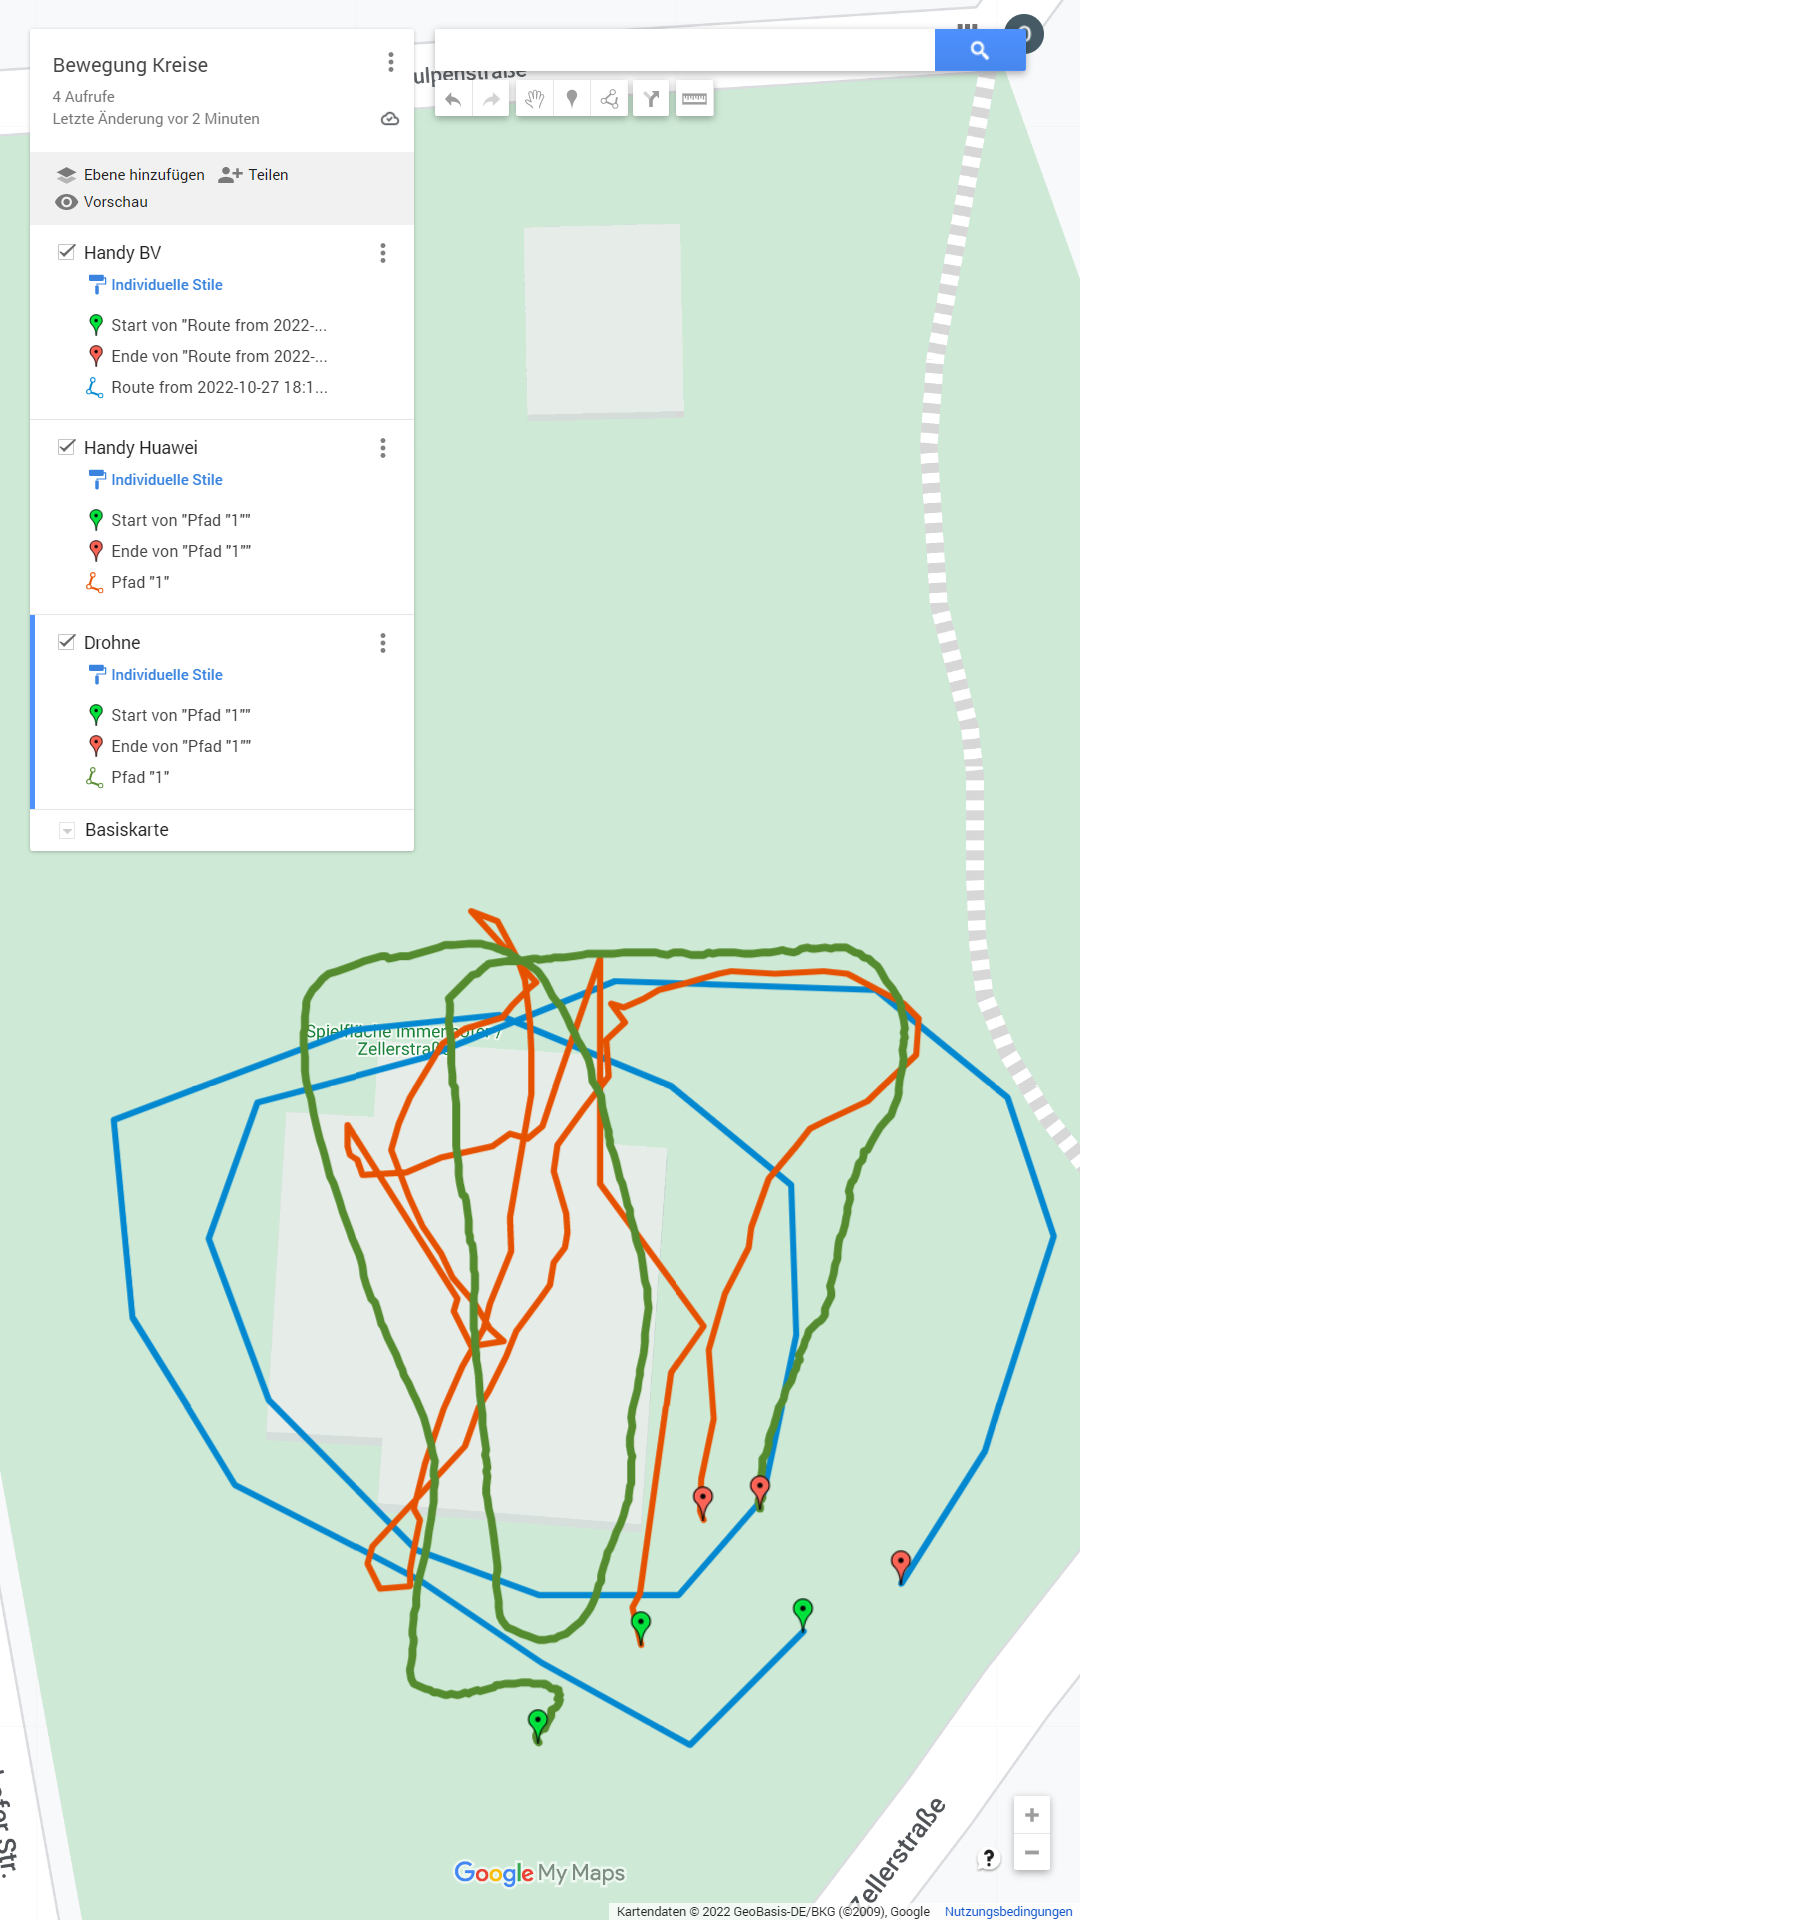
\includegraphics[width=0.5\textwidth]{images/lauf1.png}}
    \subfloat[Bewegung Bergab]{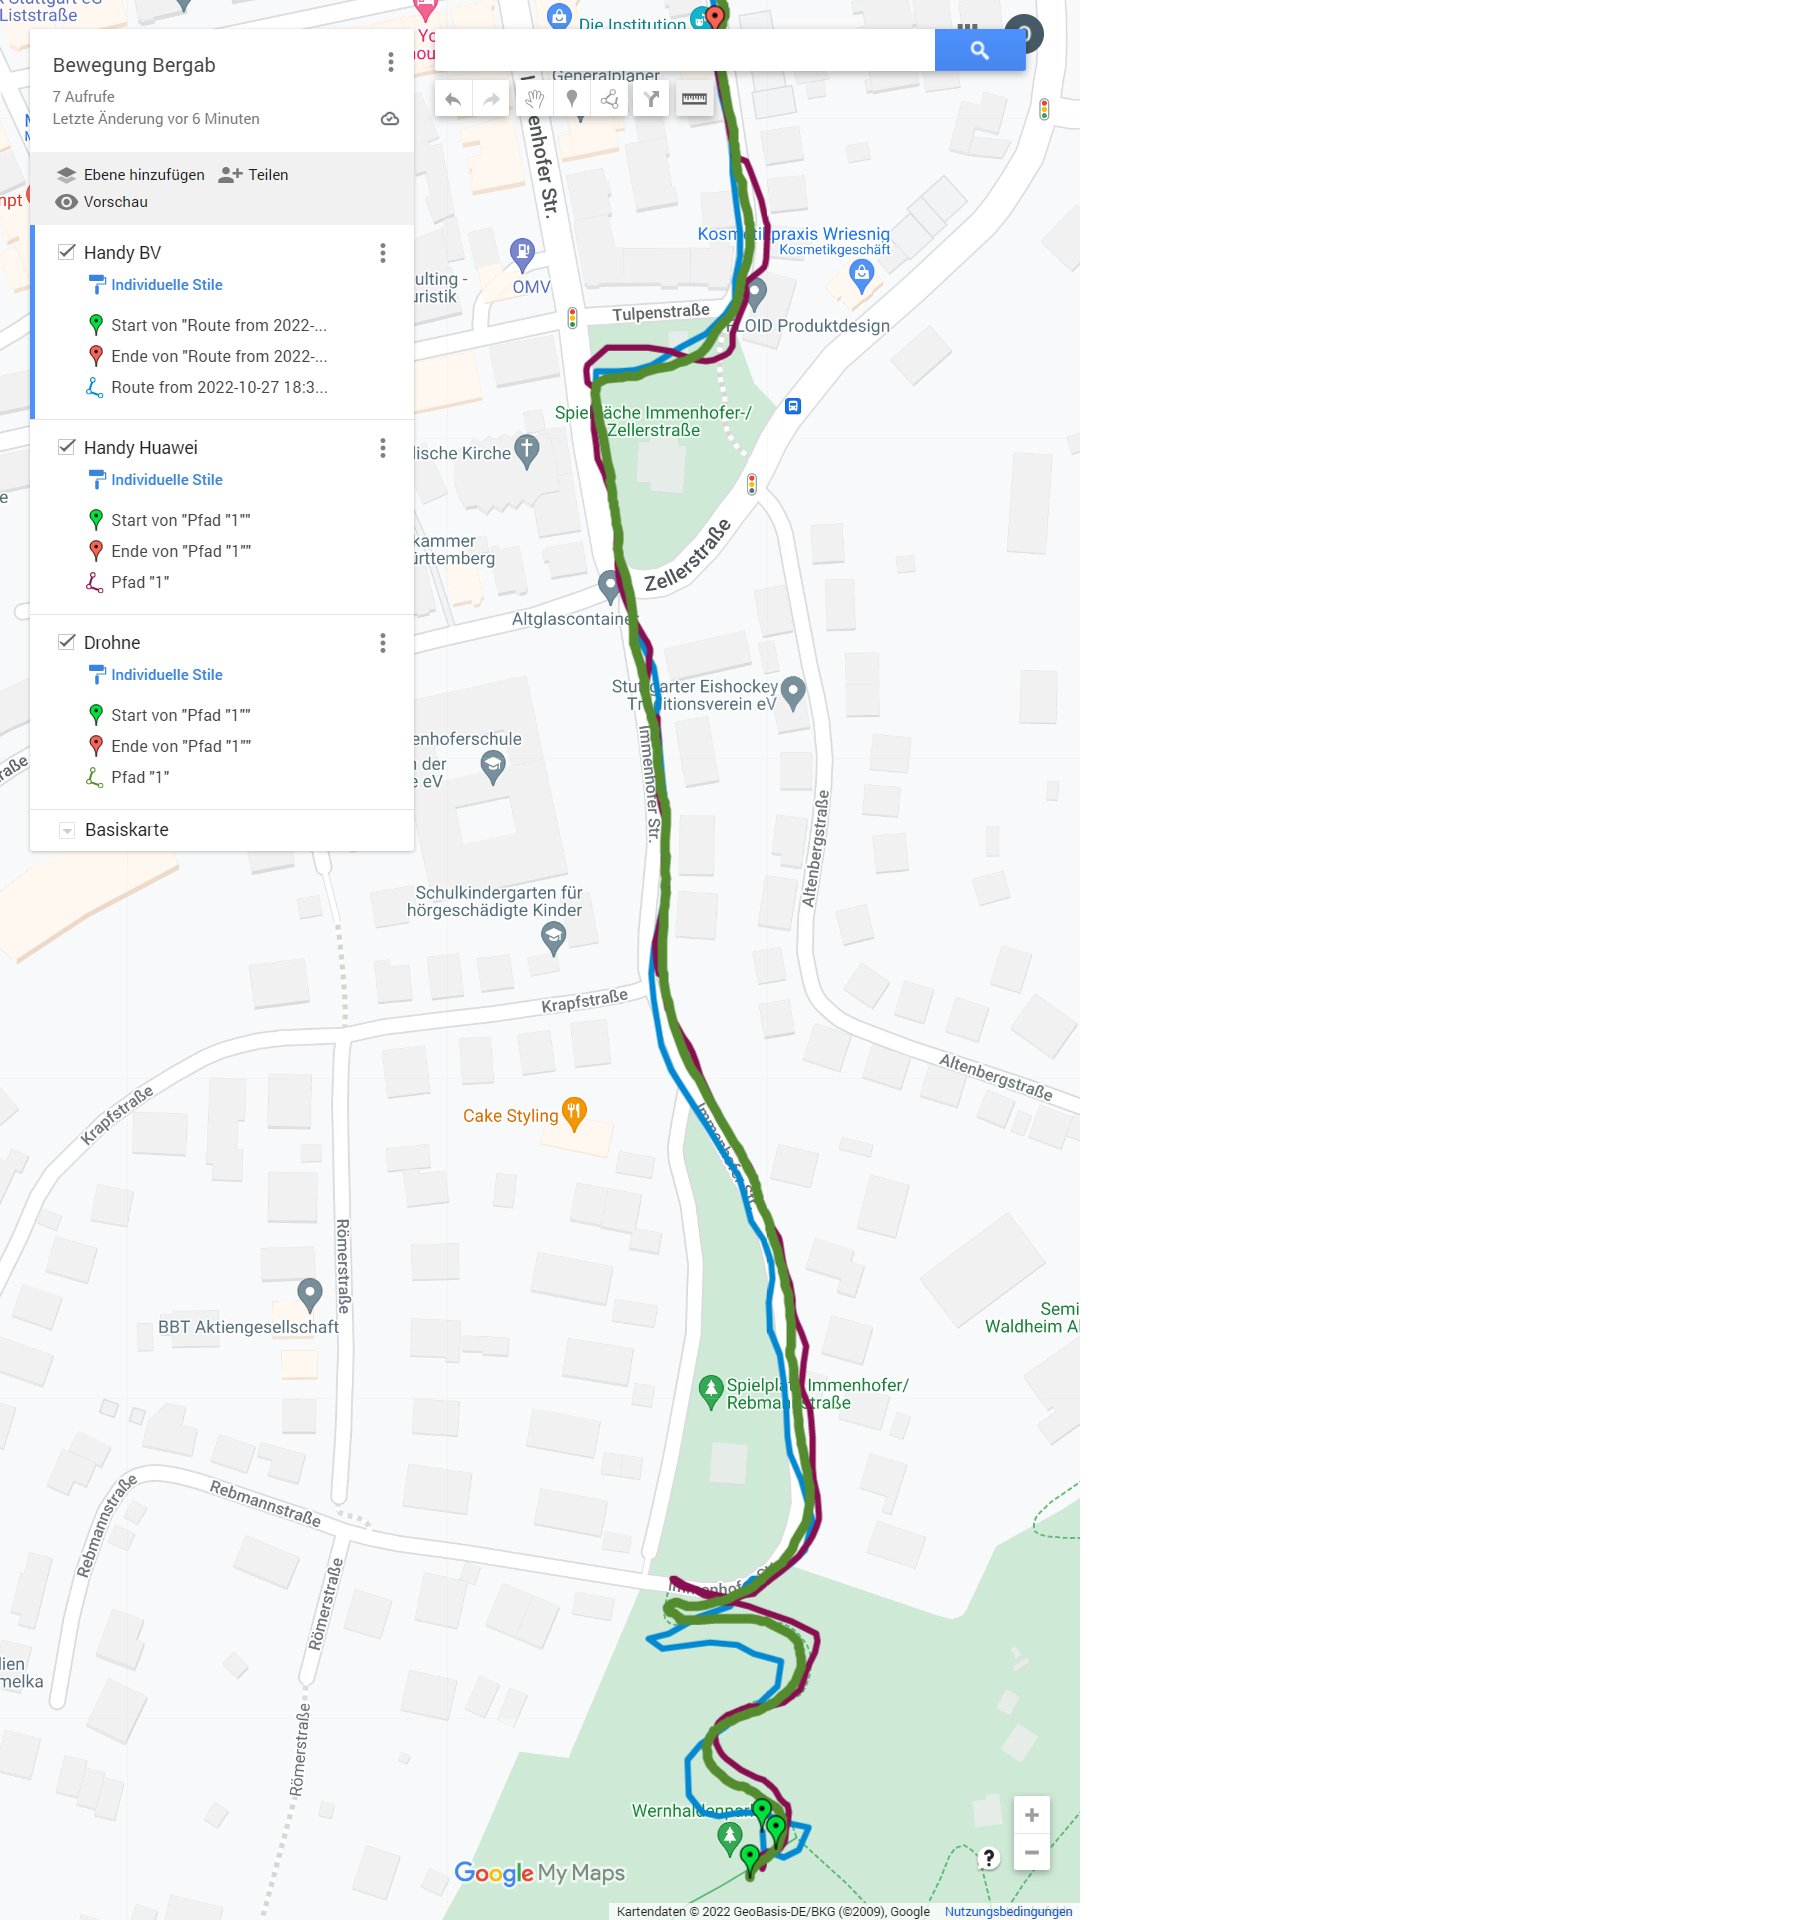
\includegraphics[width=0.5\textwidth]{images/lauf3.png}}
            
    \caption{Vergleich Bewegungsprofil verschiedener Geräte. GPS-Modul der Drohne in Grün, zwei Smartphones in Blau und Orange.}
    \label{fig:bench_gps}
\end{figure}

Weiterhin kann aus den GPS Daten Höhe, Geschwindigkeit und Neigung über die Zeit beobachtet werden. Die Drohne nimmt insgesamt mehr Messpunkte als die Smartphones auf, was ihr eine größere Genauigkeit und Zuverlässigkeit verleihen sollte. Auch gibt es bei den Smartphones teilweise Aussetzer bei der Aufzeichnung (entweder Signalverlust oder Software-Probleme). In Bild \ref{fig:bench_gps_elevation} zu sehen ist das Höhenprofil beim Bewegen der Drohne und eines Smartphones. Hätte die Drohne schwerwiegende Abweichungen während des Fluges könnte dies fatale Folgen haben. Auch ist das Profil der Drohne insgesamt ruhiger und glatter, was für gute Messwerte spricht.  

\begin{figure}[h!]
    \centering
    \subfloat[GPS-Modul Drohne]{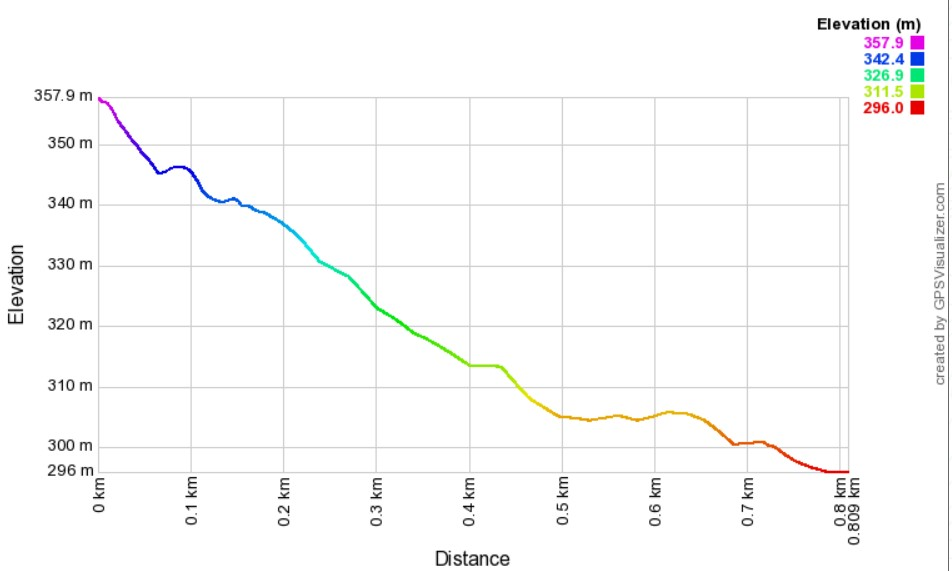
\includegraphics[width=0.5\textwidth]{images/lauf3_rpi_elevation.jpg}}
    \subfloat[Huawei-Smartphone]{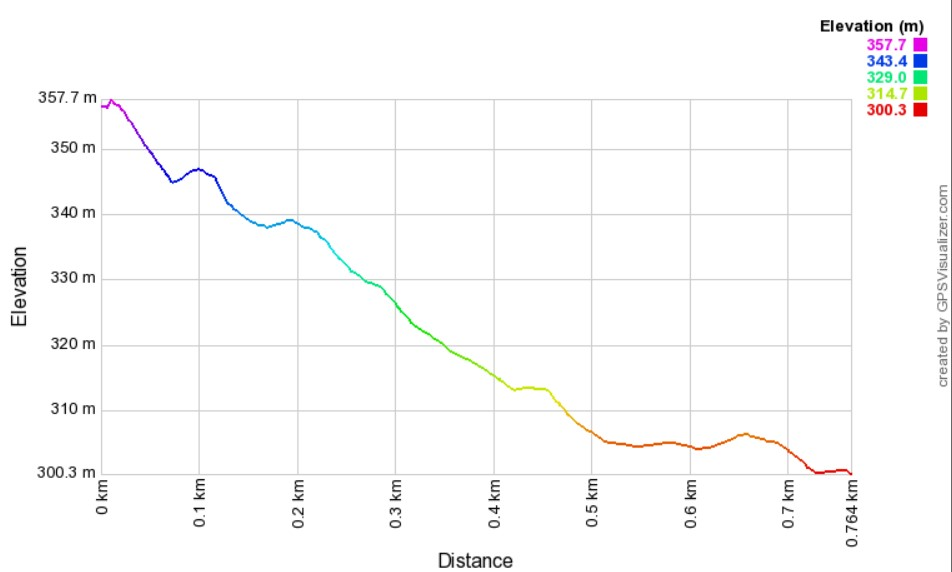
\includegraphics[width=0.5\textwidth]{images/lauf3_huawei_elevation.jpg}}
            
    \caption{Vergleich Höhenprofil verschiedener Geräte bei Bewegung bergab.}
    \label{fig:bench_gps_elevation}
\end{figure}

Um die Genauigkeit des GPS zu verbessern gibt es verschiedene Möglichkeiten\footnote{\url{https://ardupilot.org/copter/docs/common-rtk-correction.html}}. In der Praxis eingesetzt bei Landwirtschaftlichen Maschinen (Zentimetergenaue Fahrzeugführung) wird die zweite auf der Website aufgeführte Methode: über das Internet wird ein Korrektursignal abgerufen und dem GPS-Modul zugespielt. Diese Methode könnte auch einfach mithilfe des \gls{rpi} und einem GSM-Modul (Mobiles Internet über 3G) implementiert werden.

\subsection{Auslesen von Sensor-Daten}
Der Flugcontroller stellt verschiedene Sensoren bereit. Zusätzlich waren im ersten Projekt Ultraschallsensoren an den \gls{rpi} angeschlossenen. 

\subsubsection{Ultraschallsensoren am RPI}
Zuerst sollen die Ultraschall-Sensoren mit dem \gls{rpi} verbunden und getestet werden, um die Wiederverwendbarkeit zu bewerten. %Derzeit sind an der Drohne 4 Ultraschallsensoren verbaut. Davon sind zwei nach vorn gerichtet, und jeweils einer nach oben und unten. 

In \cite[Kapitel 4.3.9]{wirthErweiterungBestehendenDrohne2022} ist beschrieben dass die Signale der Sensoren mit $5V$ anliegen, aber auf $3,3V$ herabgesetzt werden müssen um die Pins des \gls{rpi} nicht zu beschädigen.
Die Beschreibung sieht vor dazu einen Spannungsteiler einzusetzen. Bei genauem betrachten des Schaltplans fällt auf, dass der Spannungsteiler falsch gebaut wurde, und nicht die gewünschte Funktion erfüllt. Um die Pins des \gls{rpi} nicht doch zu beschädigen muss eine alternative Lösung gefunden werden. 

Weiterhin wurde ein Python-Script verwendet um die Pins am \gls{rpi} zu schalten/lesen. 
Zum anstoßen einer Messung soll das Trigger-Signal für $1\mu s$ auf \texttt{HIGH} (logisch 1) gesetzt werden. Um die Zeitverzögerung zu implementieren, wurde die Funktion \enquote{wait} verwendet. Eine Messung mit dem Oszilloskop zeigt, dass besagtes \enquote{wait} im Bereich von 200us liegt.\newline
Eine ähnliche Ungenauigkeit tritt beim Auslesen des ECHO-Signals auf. Die Bibliothek des \gls{rpi} wird verwendet um die Pins zu Pollen, was den Prozessor unnötig auslastet. Messungen mit konstant eingespeister Einschaltdauer (zu messendes Signal von Signalgenerator erzeugt) ergaben, dass immer 3 von 4 Messwerten gleich, der vierte aber eine Abweichung von ca. 8\% hatte.\\
Somit kann mit Python keine genaue Messung der Ultraschallsensoren durchgeführt werden. 

\paragraph*{Verwendung eines Aurduino zum Auslesen der Sensoren}
Zur Lösung der Problemene kann bspw. zusätzlich ein Arduino verwendet werden, der die Sensordaten korrekt ausliest und digitalisiert an den \gls{rpi} weiterleitet. Dies ist eine zuverlässige Lösung, erhöht aber auch gleichzeitig den Stromverbrauch. Um die Lösung einfach zu halten, wird diese trotzdem angewandt.

Zum Senden digitaler Messwerte muss ein Protokoll verwendet werden. Die UART-Pins des \gls{rpi} sind bereits mit dem Flugcontroller verbunden. Für den Anwendungszweck bietet sich das I2C-Protokoll an. Es erlaubt eine direkte Verbindung des Arduino mit dem \gls{rpi}, denn es werden vom Arduino keine $5V$ aktiv geschalten sondern nur der Leitungsbus auf Masse heruntergezogen.

Die Ultraschallsensoren\footnote{\url{https://cdn.sparkfun.com/datasheets/Sensors/Proximity/HCSR04.pdf}} haben eine Reichweite von ca. $2cm$ bis $4m$ und eine Genauigkeit von ca. $3mm$. Für die Entwicklung wird die maximale Distanz auf $3.8m$ festgelegt. Es wird ein kleinerer Wert als im Datenblatt angenommen, da der Idealwert nur bei stillstehenden glatten Flächen erreicht werden kann. Im Datenblatt wird empfohlen, zwischen aufeinanderfolgenden Messungen mindestens $60ms$ abzuwarten, um Fehleinstreuungen durch weitere Ultraschallechos zu vermeiden. Um weitere Fehler zu vermeiden wird diese Zeit vorerst auch zwischen den Messungen der 4 Sensoren eingehalten. Eine weitere Verzögerung entsteht durch das Messen selbst (maximal $\frac{380cm}{0.5 \times 0.034\frac{cm}{s}}\approx 22352\mu s$), diese wird vorsorglich von der jeweiligen Wartezeit abgezogen. Die minimale Periode der Sensordaten beträgt somit $4 \times 60ms=240ms$. Grob gesagt, entspricht die Frequenz der Sensordaten somit $4Hz$.
%Dies ist nicht gerade hoch und könnte bei schnellen Flügen leicht zu Fehlern führen.

Ein weiteres Problem ist das durch die Ultraschallsensoren verursachte Rauschen der Messwerte. Bei Messungen im Raum mit konstantem Abstand zu Obejekten ergaben sich Abweichungen zwischen 2 Messungen von ca. $1\%-2\%$, siehe Bild \ref{fig:ultrasonic_noise}, \ref{fig:ultrasonic_scatter}. Im linken Bild sind nacheinander die Messwerte mehrerer Ultraschallsensoren aufgeführt, das rechte Bild zeigt den zeitlichen Verlauf von Messdaten. Selbst bei Stillstand (Anfang und Ende der Messung) sind Schwankungen in den Messwerten zu sehen.

Auch haben die Ultraschallsensoren ein Problem mit Bewegungen. In Bild \ref{fig:ultrasonic_scatter} wurde der Sensor zuerst in Richtung Decke gehalten (Beginn bei ca. $8s$ auf der x-Achse). Dann wurde er waagerecht gedreht, in den Raum zeigend. Kann der Sensor keinen Wert erfassen, kommt es auf dem Arduino zu einem Timeout und es wird $0$ zurückgegeben (ca. bei $11s$). Zu beachten sind die starken Abweichungen während den Bewegungen: es kommt immer wieder zu starken Einbrüchen und Anstiegen (bspw. bei $14s$) durch teilweisen Verlust des Echo-Signals.

\begin{figure}[h!]
    \centering
    \subfloat[Nacheinander ausgelesene Sensordaten]{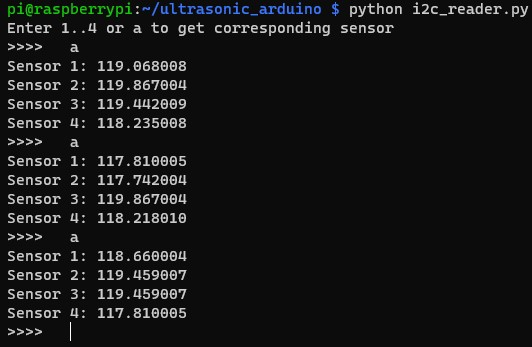
\includegraphics[width=0.5\textwidth]{images/bench_ultrasonic_noise.jpg}\label{fig:ultrasonic_noise}}
    \subfloat[Verhalten bei Bewegung eines Sensors]{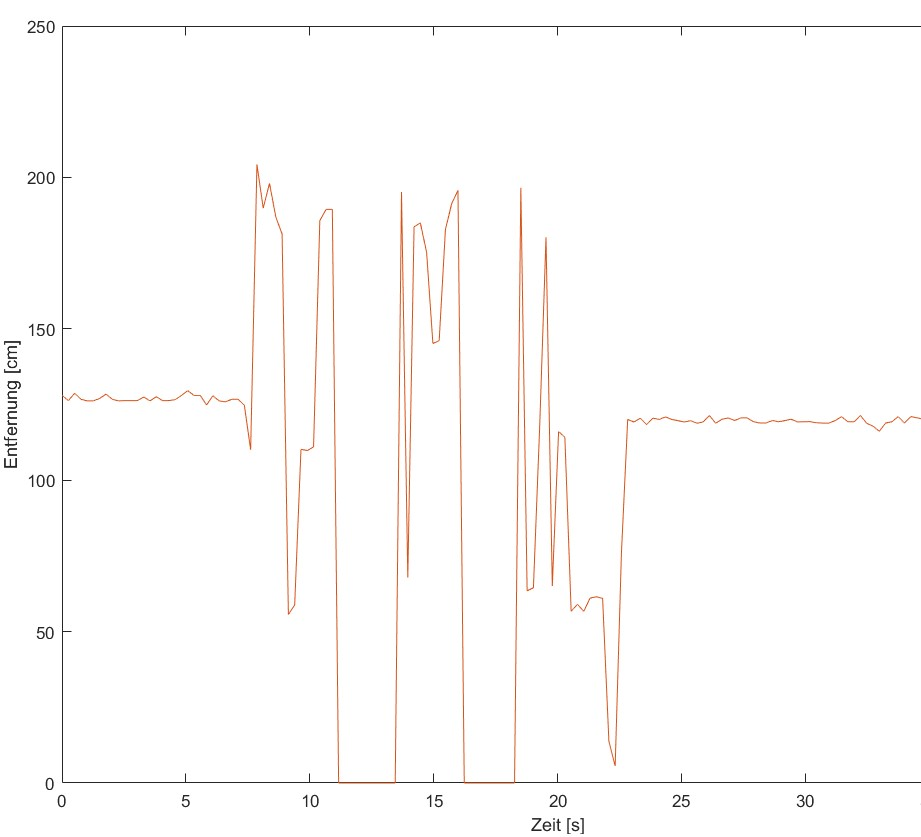
\includegraphics[width=0.5\textwidth]{images/bench_ultrasonic_movement_scatter.jpg}\label{fig:ultrasonic_scatter}}

    \caption{Demonstration der Ultraschallsensoren}
    \label{fig:ultrasonic_tests}
\end{figure}

Durch den Feldversuch wird ersichtlich, dass Ultraschallsensoren nur funktionieren, wenn sie nahezu senkrecht auf Flächen gerichtet werden. Somit können auch keine Hindernisse (wie bspw. Wände) detektiert werden, auf die sich die Drohne schräg zubewegt. Nicht messbare Entfernungen (zu nahe oder zu große Entfernung) werden beim weiteren Vorgehen durch die Entfernung von $4m$ ersetzt und die maximal messbare Entfernung der Sensoren auf $3m$ begrenzt.

Um die Messwerte der Sensoren sinnvoll verarbeiten zu können ist weiteres Filtern notwendig. Eine einfache Implementation für einen Filter sind Moving Average Filter, oder speziell für diesen Anwendungszweck, wie in \footnote{\url{https://renegaderobotics.org/filtering-sensor-data/}} beschriebene Median Filter. Bei dem zuletzt beschriebenen Verfahren werden manuell Grenzen festgelegt, welche Messwerte gefiltert werden müssen. Für die Messungen wurden Abweichungen kleiner 1\% ignoriert und größer 3\% gefiltert. Vom beschriebenen Vorgehen zum filtern wurde aber abgeichen und anstatt des Medians jeweils der Mittelwert der letzten Messwerte, gespeichert in einem Filter-Array, errechnet. In Bild \ref{fig:ultrasonic_filters} ist eine weitere Messung dargestellt. Die besten Resultate (wenige Sprünge, steile Anstiege) liefert der \enquote{Median Filter 1} und soll im Projekt weiterhin verwendet werden.

\begin{figure}[!h]
	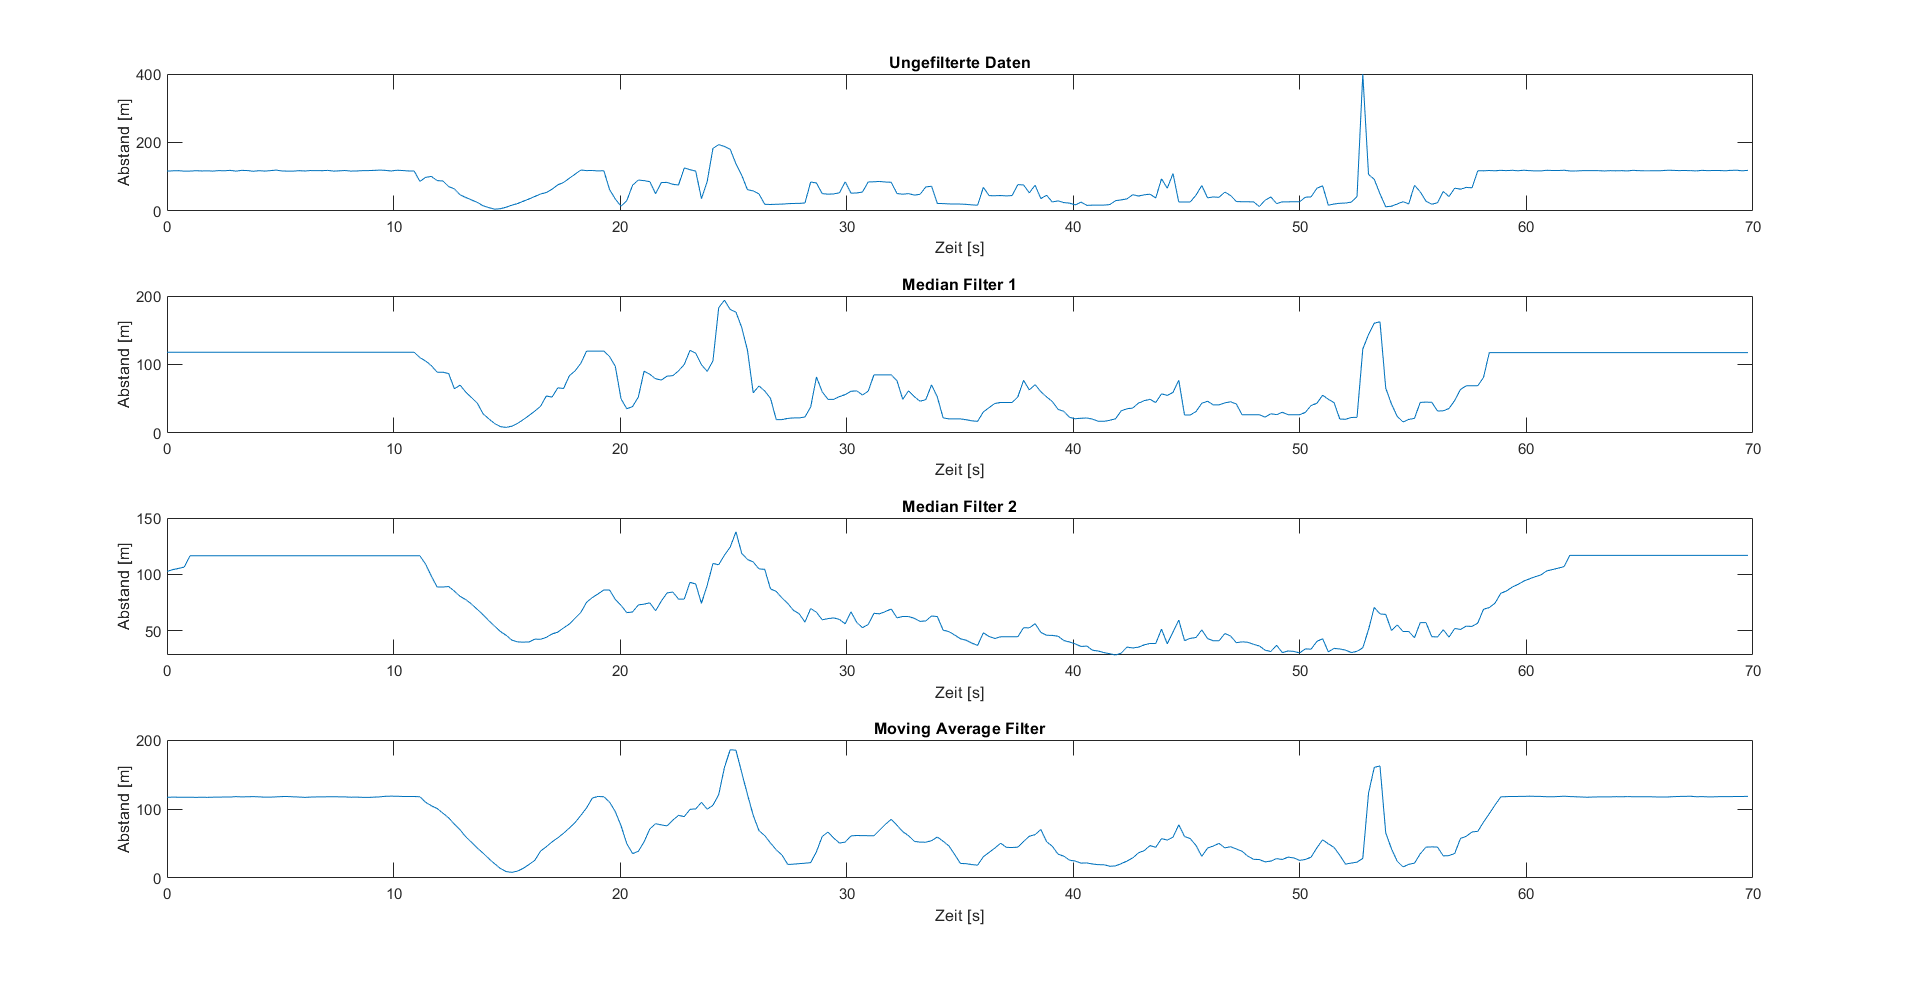
\includegraphics[width=\linewidth]{images/ultrasonic_cmp_filter.png}
	\caption{Messung mit einem Ultraschallsensor. Zu sehen: oben ungefilterte Messwerte; Median Filter 1 pflegt Sprünge in Messdaten direkt in Filter-Array ein aber berechnet Durchschnitt; Median Filter 2 pflegt berechneten Durchschnittswert in Filter-Array ein; Moving Average berechnet immer den Durchschnittswert der vergangenen Messwerte.}
	\label{fig:ultrasonic_filters}
  \end{figure} 

[TODO: neue Bibliothek entwerfen, am besten gleich mit ROS]

\subsubsection{Einspeisen von Parameterwerten der Drohne für ROS}

[TODO: vielliecht gibt es schon eine "direkte Einspeisung", muesste ich mich mal belesen]
[TODO: Alternativ kann der Flugcontroller auch einen EKF berechnen]
